% VUT FIT MITAI
% MSZ 2021/2022
% Author: Vladimir Dusek
% Login: xdusek27

%%%%%%%%%%%%%%%%%%%%%%%%%%%%%%%%%%%%%%%%%%%%%%%%%%%%%%%%%%%%%%%%%%%%%%%%%%%%%%%%

% Path to figures
\graphicspath{{tin/nerozhodnutelnost/figures}}

%%%%%%%%%%%%%%%%%%%%%%%%%%%%%%%%%%%%%%%%%%%%%%%%%%%%%%%%%%%%%%%%%%%%%%%%%%%%%%%%

\chapter{TIN~--~Nerozhodnutelnost (problém zastavení TS, princip diagonalizace a redukce, Postův korespondenční problém).}

%%%%%%%%%%%%%%%%%%%%%%%%%%%%%%%%%%%%%%%%%%%%%%%%%%%%%%%%%%%%%%%%%%%%%%%%%%%%%%%%

\section{Zdroje}

\begin{compactitem}
    \item \path{tin_2021_merged.pdf}
    \item \path{TIN_2020-11-03.mp4}
    \item \path{TIN_2020-11-10.mp4}
    \item \path{TIN_2020-11-20_demo.mp4}
\end{compactitem}

%%%%%%%%%%%%%%%%%%%%%%%%%%%%%%%%%%%%%%%%%%%%%%%%%%%%%%%%%%%%%%%%%%%%%%%%%%%%%%%%

\section{Rozhodovací problém}

\paragraph*{Rozhodovací problém}

\begin{compactitem}
    \item Rozhodovací problém (\textit{decision problem}) $P$ může být chápán jako funkce $f_P$ s oborem hodnot $\{ true, false \}$.

    \item Rozhodovací problém je obvykle specifikován: \begin{compactitem}
        \item definičním oborem $A_P$ reprezentujícím množinu možných instancí problému,

        \item podmnožinou $B_P \subseteq A_P$, $B_P = \{ p ~|~ f_P(p) = true \}$ instancí, pro které je hodnota $f_P$ rovna $true$.
    \end{compactitem}
\end{compactitem}

\paragraph*{Kódování problémů}

\begin{compactitem}
    \item V teorii formálních jazyků používáme ke kódování jednotlivých instancí problémů řetězce nad vhodnou abecedou $\Sigma$.

    \item Pak je rozhodovací problém $P$ přirozeně specifikován
    jazykem $L_P = \{ w \in \Sigma^* ~|~ w = code(p),~ p \in B_P \}$, kde $code: A_P \rightarrow \Sigma^*$ je injektivní funkce, která přiřazuje instancím problému příslušný řetězec (nezávisle na $f_P$).
\end{compactitem}

\paragraph*{Rozhodování problémů TS}

\begin{compactitem}
    \item Nechť $P$ je problém specifikovaný jazykem $L_P$ nad abecedou $\Sigma$. Problém P nazveme: \begin{compactitem}

        \item \textbf{Rozhodnutelný}, pokud $L_P$ je rekurzívní jazyk, tj. existuje TS, který $L_P$ rozhoduje (přijme každý řetězec $w \in L_P$, a zamítne každý řetězec $w \in \Sigma^* - L_P $).

        \item \textbf{Nerozhodnutelný}, když není rozhodnutelný.

        \item \textbf{Částečně rozhodnutelný}, jestliže LP je rekurzívně vyčíslitelný jazyk.

    \end{compactitem}

    \item Z toho plyne, že každý rozhodnutelný problém je současně částečně rozhodnutelný, ale některé nerozhodnutelné problémy nejsou ani částečně rozhodnutelné. \begin{compactitem}
        \item Problém je nerozhodnutelný, pokud pro něj neexistuje úplný turingův stroj.
    \end{compactitem}
\end{compactitem}

% Zjistit jestli turingův stroj je úplný, je taky problém.

\begin{figure}[H]
    \centering
    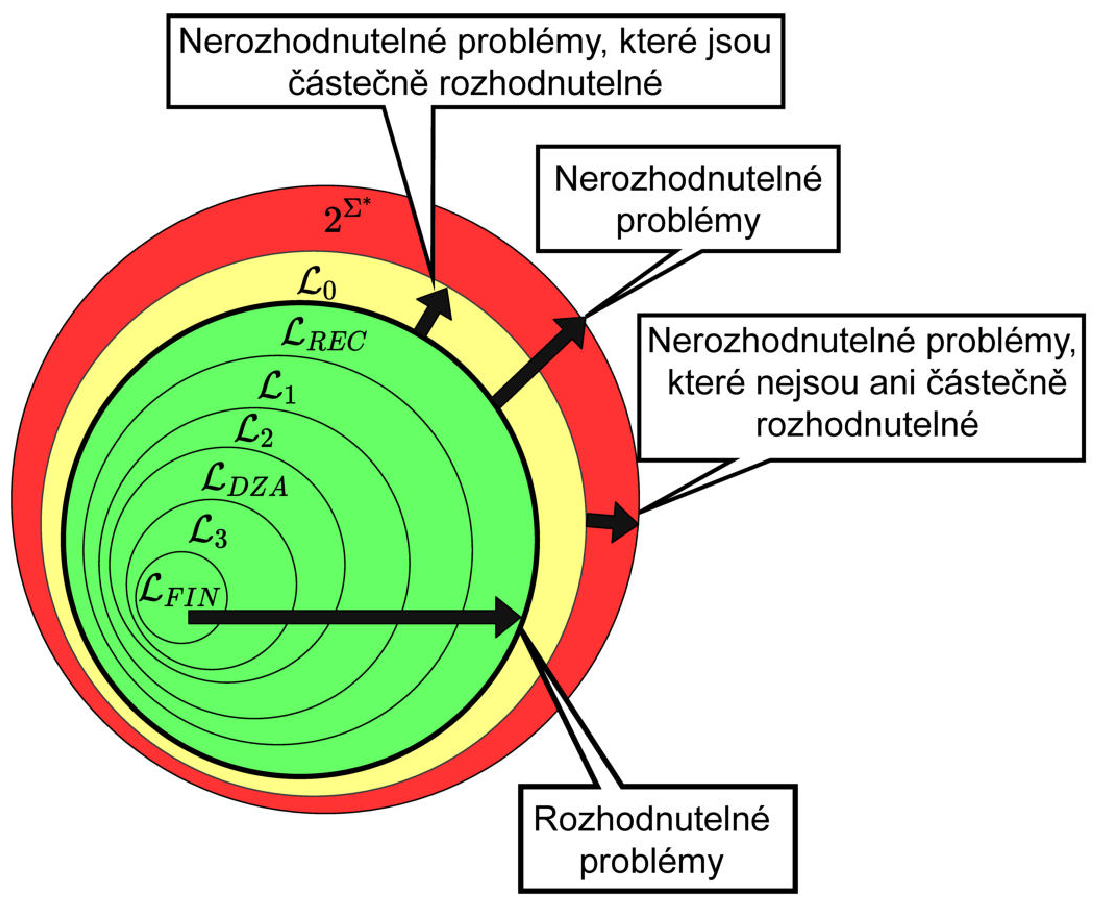
\includegraphics[width=0.9\linewidth]{fj_hierarchy.pdf}
    \caption{Hierarchie jazýků/problémů a jejich (ne)rozhodnutelnost.}
\end{figure}

%%%%%%%%%%%%%%%%%%%%%%%%%%%%%%%%%%%%%%%%%%%%%%%%%%%%%%%%%%%%%%%%%%%%%%%%%%%%%%%%

\section{Známé problémy}

\subsection*{Problém zastavení TS}

\begin{compactitem}
    \item Problém zastavení TS $M$ na daném vstupu $w$ (HP, \textit{Halting Problem}).

    \item Neformálně: Znáte-li zdrojový kód programu (TS) a jeho vstup, rozhodněte, zda program zastaví, nebo zda poběží navždy bez zastavení.

    \item Problém není rozhodnutelný, ale je částečně rozhodnutelný. \begin{compactitem}
        \item $HP \in \mathcal{L}_{RE}$
        \item Důkaz: s využitím Cantorovy diagonalizace.
    \end{compactitem}

\end{compactitem}

$$ HP = \{ \langle M \rangle \# \langle w \rangle ~|~ \text{TS M na vstupu w zastaví} \} $$

\subsection*{Problém nezastavení TS}

\begin{compactitem}
    \item Problém nezastavení TS $M$ na daném vstupu $w$ (co-HP, \textit{co-Halting Problem}).

    \item Neformálně: Znáte-li zdrojový kód programu (TS) a jeho vstup, rozhodněte, zda program nezastaví (poběží navždy bez zastavení), nebo zda zastaví.

    \item Problém není ani částečně rozhodnutelný. \begin{compactitem}
        \item $coHP \not\in \mathcal{L}_{RE}$
        \item Důkaz: vyplývá z definice komplementu.
    \end{compactitem}
\end{compactitem}

$$ coHP = \{ \langle M \rangle \# \langle w \rangle ~|~ \text{TS M na vstupu w nezastaví} \} $$

\subsection*{Problém náležitosti}

\begin{compactitem}
    \item Problém náležitosti řetězce $w$ do jazyka $L$, $L \in \mathcal{L}_0$ (MP, \textit{Membership Problem}).

    \item Neformálně: Znáte-li TS a jeho vstup, rozhodněte, zda TS daný vstup přijme (zastaví a akceptuje) a nebo nepřijme (zastaví a neakceptuje, zastaví abnormálně, nezastaví). \begin{compactitem}
        \item Jde o podobný případ jako problém zastavení TS, pouze obsahuje krok navíc.
    \end{compactitem}

    \item Problém není rozhodnutelný, ale je částečně rozhodnutelný. \begin{compactitem}
        \item $MP \in \mathcal{L}_{RE}$
        \item Důkaz: s využitím redukce z HP.
    \end{compactitem}
\end{compactitem}

$$ MP = \{ \langle M \rangle \# \langle w \rangle ~|~ w \in L(M) \} $$

\subsection*{Problém nenáležitosti}

\begin{compactitem}
    \item Problém nenáležitosti řetězce $w$ do jazyka $L$, $L \in \mathcal{L}_0$ (coMP, \textit{Non-Membership Problem}).

    \item Neformálně: Znáte-li TS a jeho vstup, rozhodněte, zda TS daný vstup nepřijme (zastaví a neakceptuje, zastaví abnormálně, nezastaví) a nebo přijme (zastaví a akceptuje).

    \item Problém není ani částečně rozhodnutelný. \begin{compactitem}
        \item $coMP \not\in \mathcal{L}_{RE}$
        \item Důkaz: s využitím redukce z coHP.
    \end{compactitem}

\end{compactitem}

$$ coMP = \{ \langle M \rangle \# \langle w \rangle ~|~ w \not\in L(M) \} $$

\subsection*{Postův korespondenční problém}

\begin{compactitem}
    \item Postův systém $S$ nad abecedou $\Sigma$ je dán neprázdným seznamem dvojic neprázdných řetězců nad $\Sigma$, formálně: $$ S = \langle (\alpha_1 , \beta_1), \dots, (\alpha_k , \beta_k) \rangle, \text{ pro } k \geq 1, \forall i : 1 \leq i \leq k : \alpha_i, \beta_i \in \Sigma^+ $$

    \item Řešením Postova systému $S$ je každá neprázdná posloupnost přirozených čísel $I = \langle i_1, i_2, \dots, i_m \rangle$, kde $m \geq 1$ a $1 \leq j \leq m : 1 \leq i_j \leq k$, tak, že: $$ \alpha_{i_1}, \alpha_{i_2}, \dots, \alpha_{i_m} = \beta_{i_1}, \beta_{i_2}, \dots, \beta_{i_m} $$ \begin{compactitem}
        \item $m$ není omezené a indexy se mohou opakovat.
    \end{compactitem}

    \item Postův korespondenční problém (PCP) zní: existuje pro daný Postův systém řešení?

    \item Problém není ani částečně rozhodnutelný. \begin{compactitem}
        \item $PCP \not\in \mathcal{L}_{RE}$
        \item Důkaz: \textit{nezkouší se}
    \end{compactitem}

    \item Příklad: PS $S$ nad $\Sigma = \{ a, b \}$: \begin{compactitem}
        \item $S = \langle (ab, a), (aa, baaab), (aa, a) \rangle$
        \item $S$ má řešení, např. $I = \langle 1, 2, 1, 3\rangle$ \begin{compactitem}
            \item $ab . aa . ab . aa = a . baaab . a . a$
        \end{compactitem}
    \end{compactitem}

\end{compactitem}

\subsection*{Další problémy} \begin{compactitem}
    \item $ \{ \langle M \rangle ~|~ \text{TS M má aspoň 2020 stavů } \} \in \mathcal{L}_{Rec}$

    \item $ \{ \langle M \rangle ~|~ \text{TS M učiní více než 2020 kroků na vstupu } \epsilon \} \in \mathcal{L}_{Rec}$

    \item $ \{ \langle M \rangle ~|~ \text{TS M učiní více než 2020 kroků na nějakém vstupu } \} \in \mathcal{L}_{Rec}$

    \item $ \{ \langle M \rangle ~|~ L(M) \not= \emptyset \} \in \mathcal{L}_{RE}$

    \item $ \{ \langle M \rangle ~|~ |L(M)| \geq 42 \} \in \mathcal{L}_{RE}$

    \item $ \{ \langle M \rangle ~|~ L(M) = \emptyset \} \not\in \mathcal{L}_{RE}$

    \item $ \{ \langle M \rangle ~|~ |L(M)| \leq 42 \} \not\in \mathcal{L}_{RE}$

    \item $ \{ \langle M \rangle ~|~ L(M) \in \mathcal{L}_{Rec} \} \not\in \mathcal{L}_{RE}$
\end{compactitem}

%%%%%%%%%%%%%%%%%%%%%%%%%%%%%%%%%%%%%%%%%%%%%%%%%%%%%%%%%%%%%%%%%%%%%%%%%%%%%%%%

\section{Diagonalizace}

\begin{compactitem}
    \item Diagonalizace (Cantorova diagonální metoda) je důkázová technika sporem, která slouží k porovnání mohutnosti dvou množin (zejména dvou nekonečných množin).

    \item Spočetné nekonečno: \begin{compactitem}
        \item Dokážeme \uv{spočítat} a uspořádat.
        \item Existuje bijekce mezi množinou $\mathbb{N}$ a každou spočetně nekonečnou množinou.
    \end{compactitem}

    \item Nespočetné nekonečno: \begin{compactitem}
        \item Nedokážeme \uv{spočítat} a uspořádat.
        \item Neexistuje bijekce mezi množinou $\mathbb{N}$ a žádnou nespočetně nekonečnou množinou.
    \end{compactitem}
\end{compactitem}

\subsection*{Příklad 1: dokažte, že $\mathbb{R}$ je větší než $\mathbb{N}$}

\begin{compactitem}
    \item Zřejmě platí, že pokud podmnožiny množiny je nespočetná, tak i množina je nespočetná. \begin{compactitem}
        \item Z toho vyplývá, že stačí dokázat že libovolná podmnožina $M \subseteq \mathbb{R}$ je nespočetná.
        \item Vybereme množinu $M = (0, 1)$.
    \end{compactitem}

    \item Předpokládejme, že $M$ je spočetná množina, pak existuje bijekce $f : \mathbb{N} \leftrightarrow M$.

    \item Uspořádejme $M$ do libovolné posloupnosti a zobrazme $f$ jako nekonečnou matici.

    \begin{table}[H]
        \begin{tabular}{l|llll}
                   & 1. desetinná pozice & 2. desetinná pozice & 3. desetinná pozice & \dots \\ \hline
            $f(0)$ & $d_{11}$            & $d_{12}$            & $d_{13}$            & \dots \\
            $f(1)$ & $d_{21}$            & $d_{22}$            & $d_{23}$            & \dots \\
            $f(2)$ & $d_{31}$            & $d_{32}$            & $d_{33}$            & \dots \\
            \dots  & \dots               & \dots               & \dots               & \dots \\
        \end{tabular}
        \caption*{Kde $\forall i,j : d_{ij} \in \{ 0, 1, \dots, 9 \}$ a $\forall n \in \mathbb{N} : f(n) = 0, d_{n1} d_{n2} \dots$}
    \end{table}

    \item Uvažme číslo $x = 0, e_1 e_2 e_3 \dots$ takové, že $e_i = 9 - d_ii$ pro $i = 1, 2, 3, \dots$.

    \item Zřejmě platí, že $x \in M$ a tedy, musí existovat $n \in \mathbb{N} : f(n) = x$.

    \item Ale současně $\forall n \in \mathbb{N} : f(n) \not= x$ protože dojde k neshodě minimálně na diagonále. \begin{compactitem}
        \item Spor.
    \end{compactitem}
\end{compactitem}

\subsection*{Příklad 2: dokažte, že $2^{\Sigma^*}$ je větší než $\mathcal{L}_0$}

% Jazyků je nespočetně mnoho.

% Ale všech možný programů (TS) je spočetně mnoho, proč? Protože kódování TS je možné interpretovat jako přirozené číslo. A těch je spočetně mnoho.

\begin{figure}[H]
    \centering
    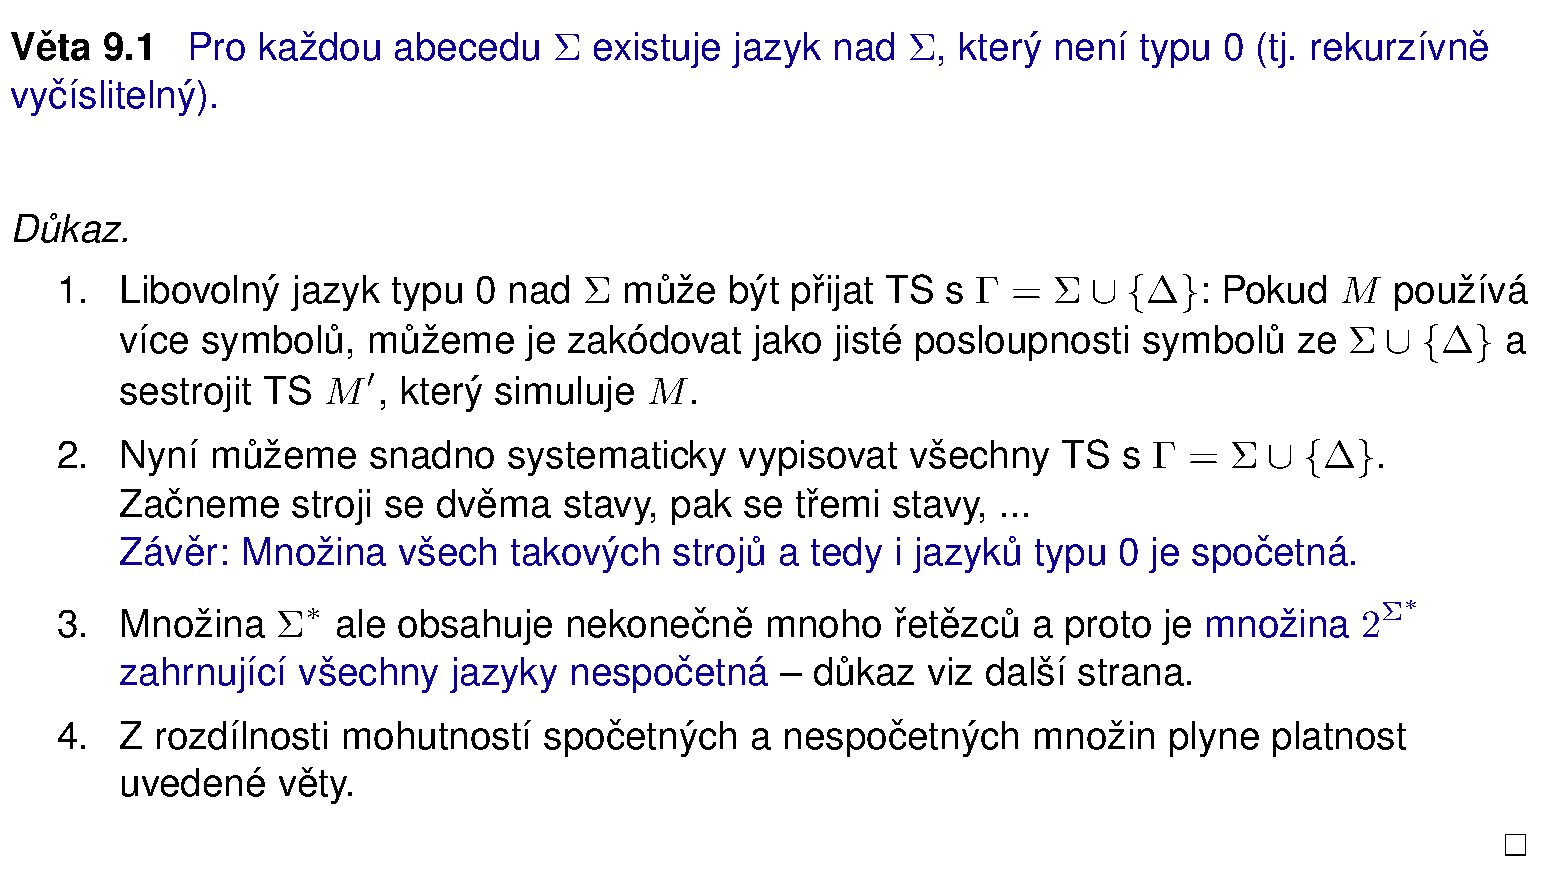
\includegraphics[width=1\linewidth]{diagonalizace_pr2_p1.pdf}
\end{figure}

\begin{figure}[H]
    \centering
    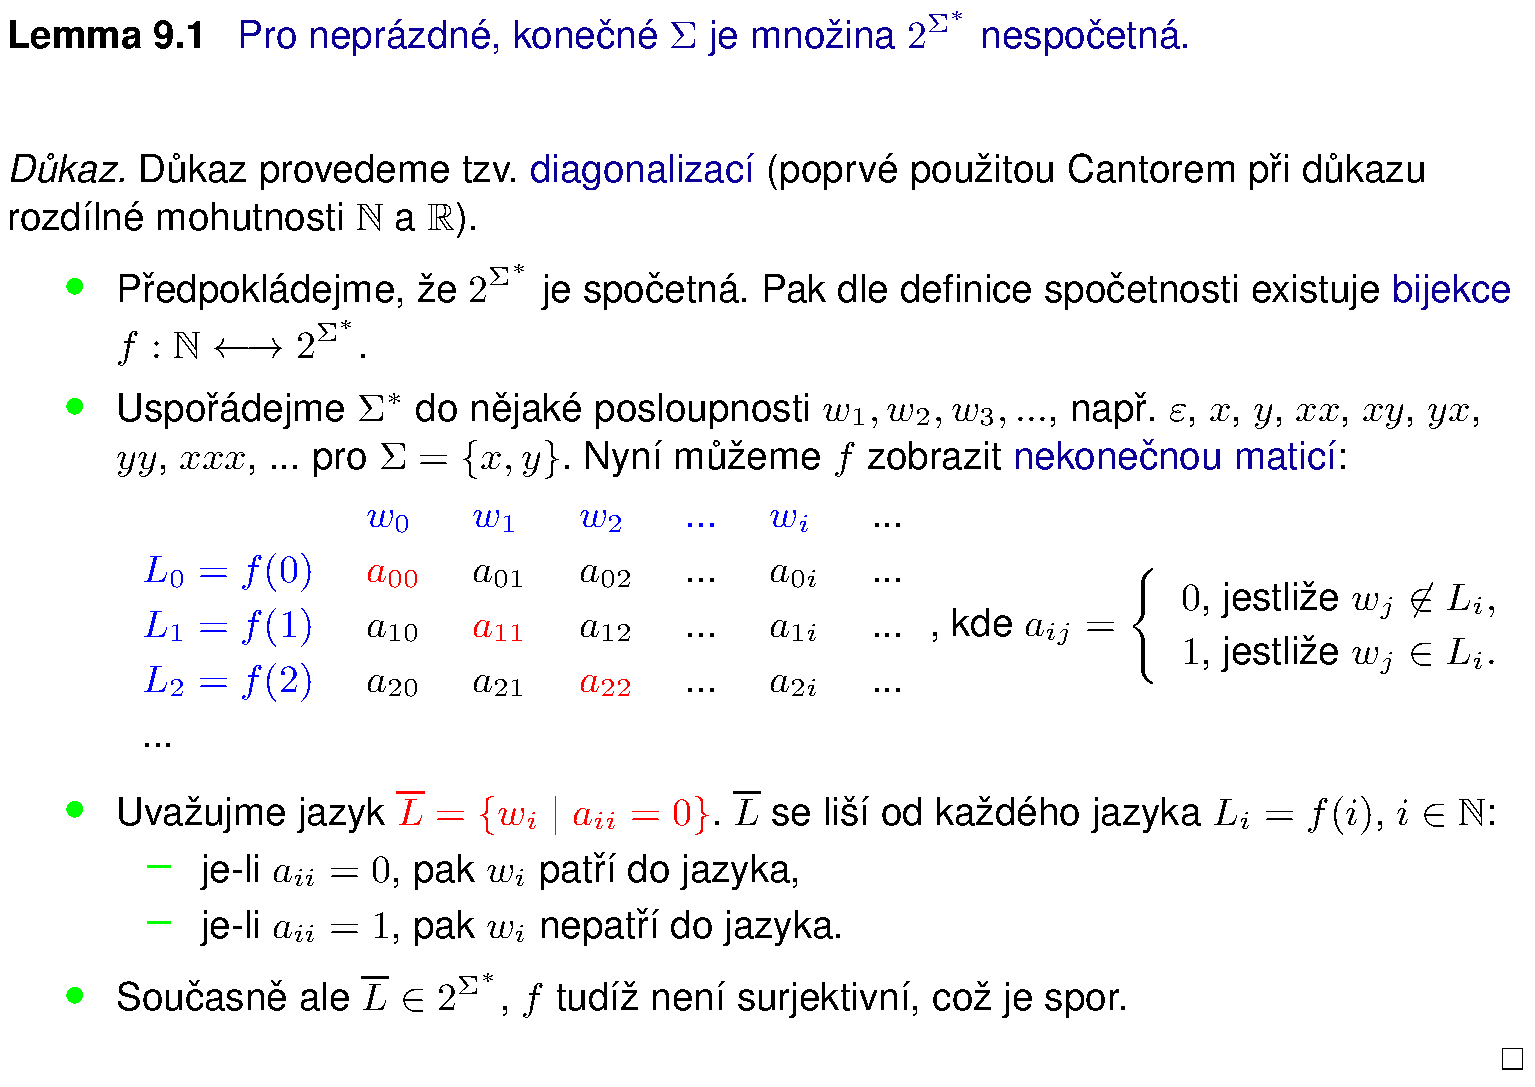
\includegraphics[width=1\linewidth]{diagonalizace_pr2_p2.pdf}
\end{figure}

\subsection*{Příklad 3: dokažte, že HP není rozhodnutelný, ale je částečně rozhodnutelný}

\begin{figure}[H]
    \centering
    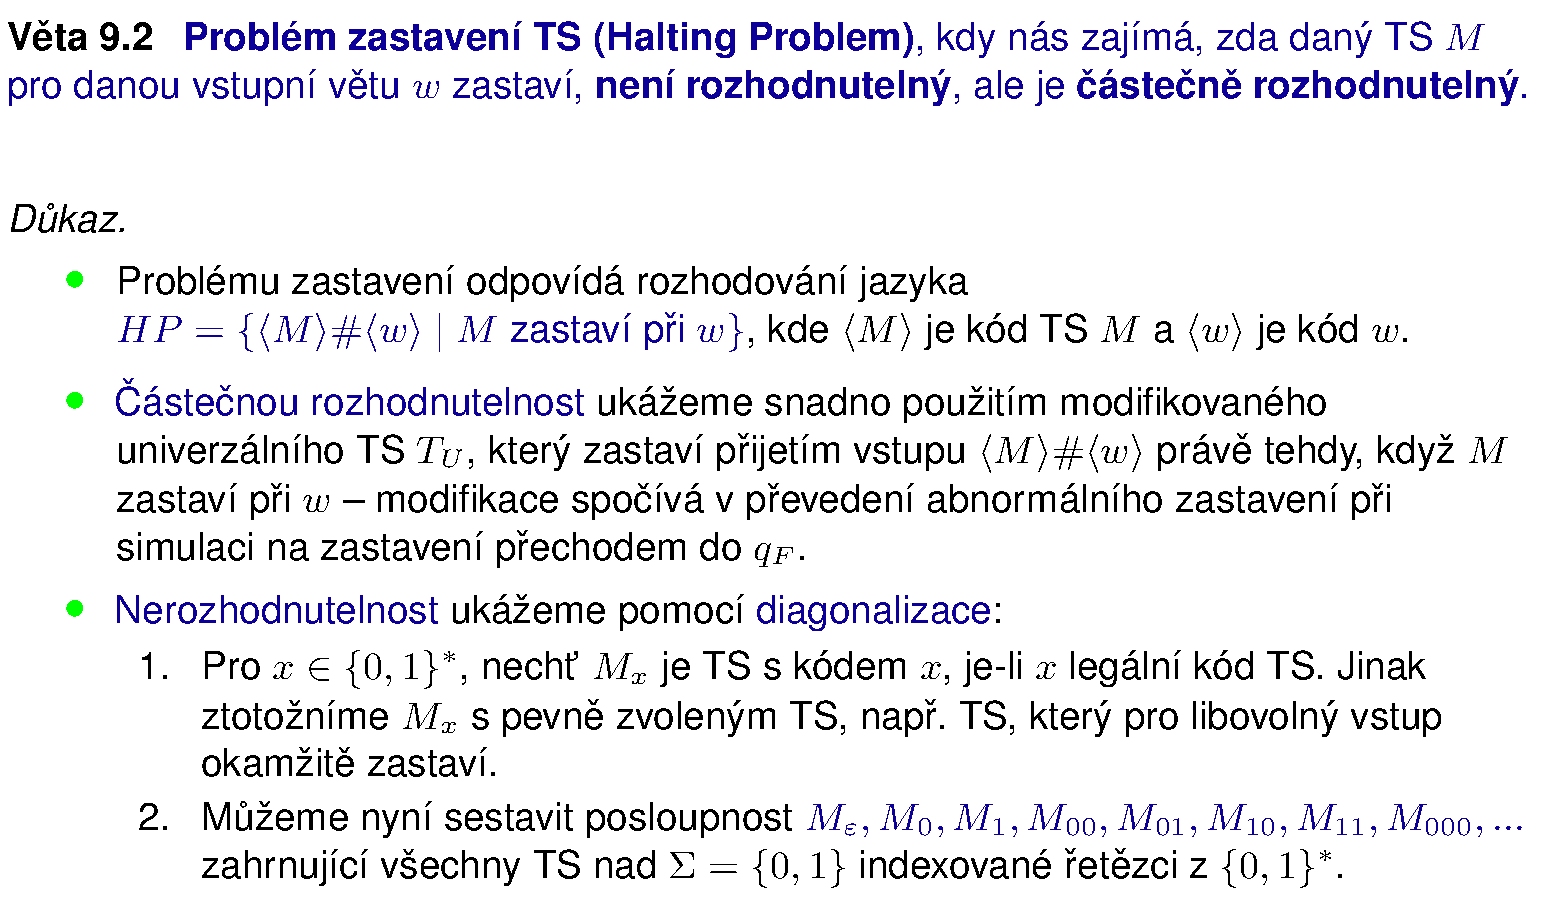
\includegraphics[width=1\linewidth]{diagonalizace_pr3_p1.pdf}
\end{figure}

\begin{figure}[H]
    \centering
    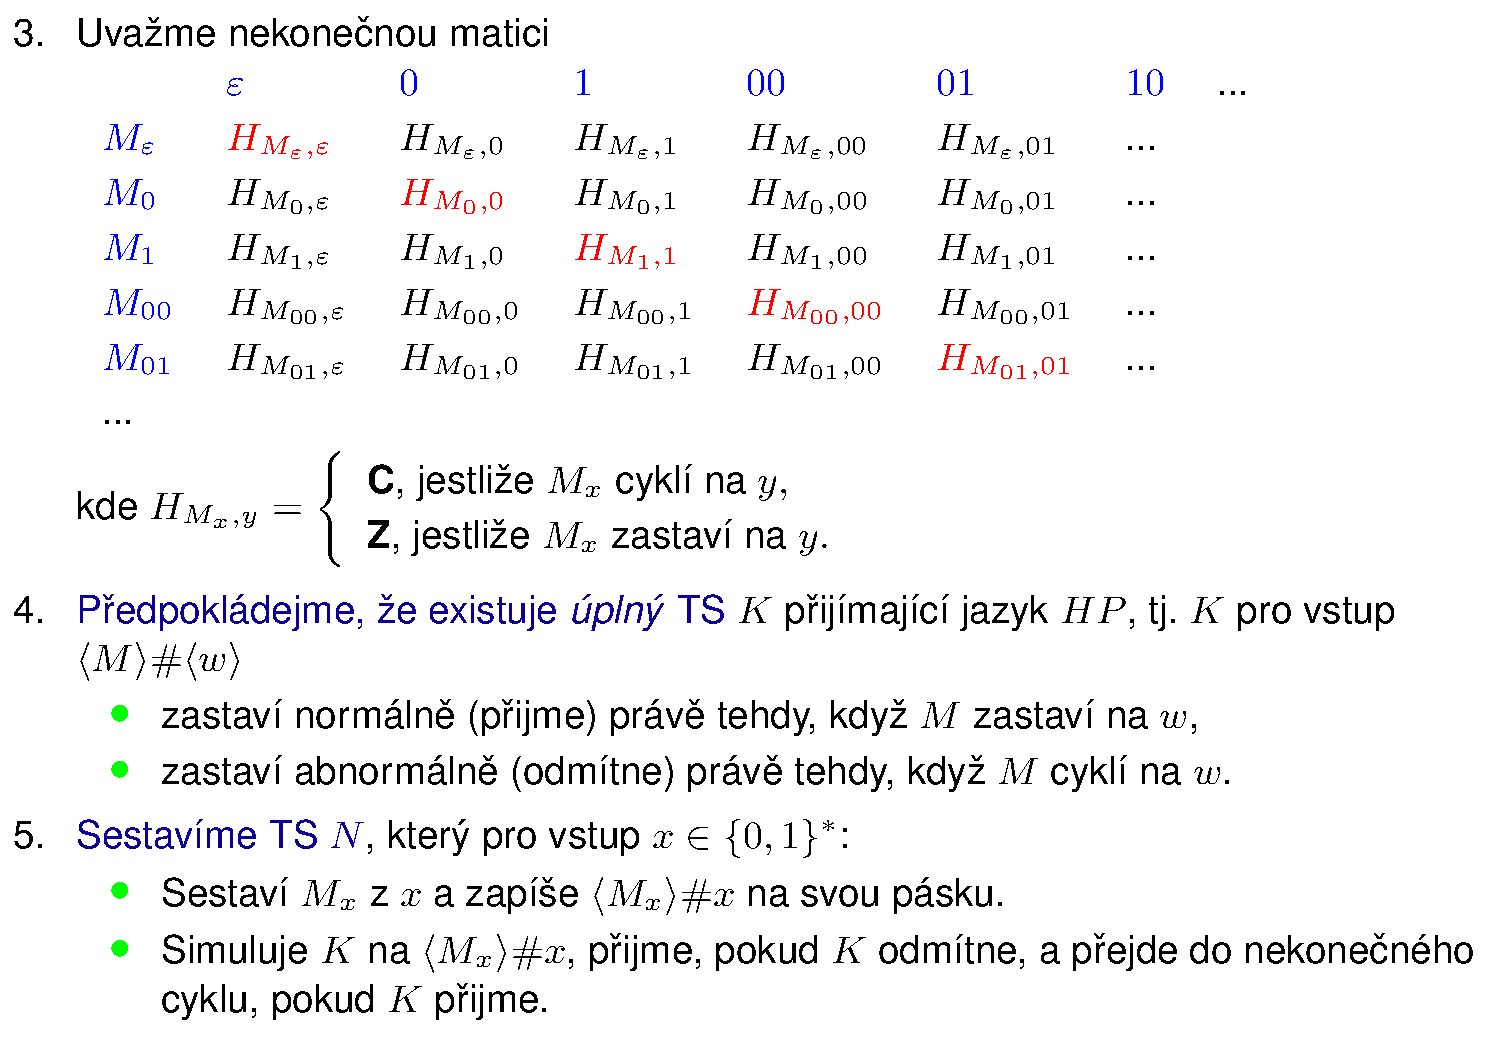
\includegraphics[width=1\linewidth]{diagonalizace_pr3_p2.pdf}
\end{figure}

\begin{figure}[H]
    \centering
    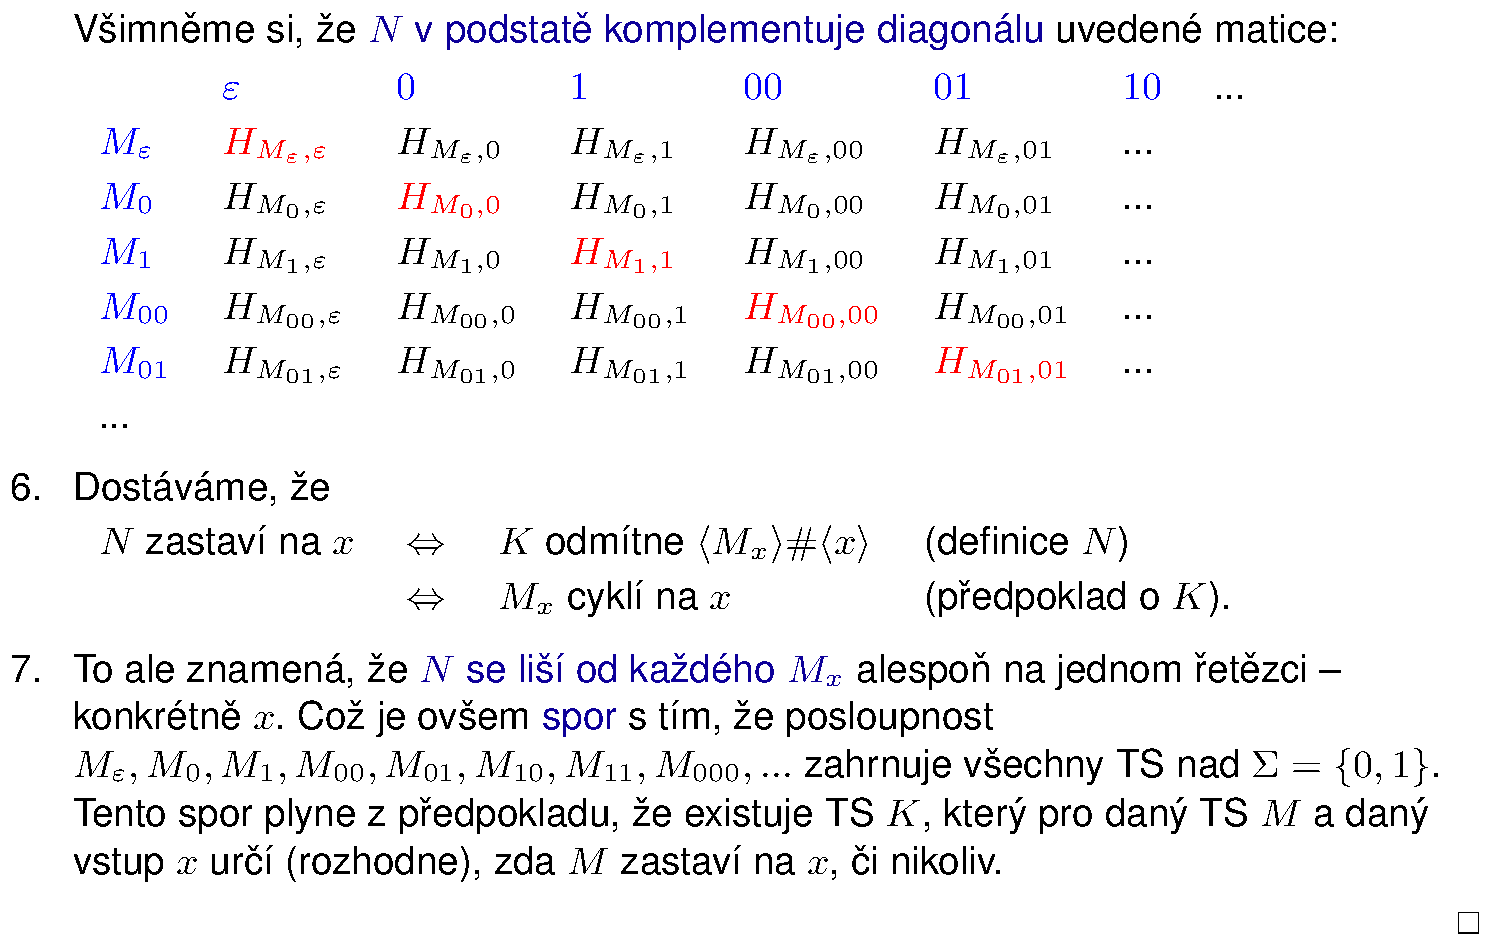
\includegraphics[width=1\linewidth]{diagonalizace_pr3_p3.pdf}
\end{figure}

\begin{figure}[H]
    \centering
    
\includegraphics[width=1\linewidth]{diagonalizace_pr3_p4.pdf}
\end{figure}

%%%%%%%%%%%%%%%%%%%%%%%%%%%%%%%%%%%%%%%%%%%%%%%%%%%%%%%%%%%%%%%%%%%%%%%%%%%%%%%%

\section{Redukce}

\begin{compactitem}
    \item Redukce je důkazová technika, která slouží k dokázání, že nějaký problém není rozhodnutelný (částečně rozhodnutelný)~--~neboli, že určitý jazyk není rekurzívní (rekurzívně vyčíslitelný). \begin{compactitem}
        \item Víme, že jazyk $A$ není rekurzívní (rekurzívně vyčíslitelný) a zkoumáme jazyk $B$. Ukážeme, že $A$ lze úplným TS převést (redukovat) na $B$, to ale znamená, že $B$ rovněž není rekurzivní (rekurzívně vyčíslitelný)~--~jinak by šlo použít úplný TS (ne-úplný TS) přijímající $B$ a příslušné redukce k sestavení úplného TS (ne-úplného TS) přijímajícího $A$, což by byl spor.
    \end{compactitem}

    \item Redukce vytváří uspořádání na problémech (nějaký problém je aspoň tak těžký jako jiný problém).

    % \item Existuje-li redukce jazyka $A$ na $B$, říkáme, že $A$ je redukovatelný na $B$, což značíme $A \leq B$.
\end{compactitem}

\paragraph*{Definice} Mějme jazyky $L_1 \subseteq \Sigma_1^*$ a $L_2 \subseteq \Sigma_2^*$. Redukce jazyka $L_1$ na jazyk $L_2$ je funkce $\sigma : \Sigma_1^* \rightarrow \Sigma_2^*$ taková, že \begin{compactitem}
    \item $\sigma$ je implementovatelná úplným TS (totální rekurzivně vyčíslitelná funkce),
    \item $\forall w \in \Sigma_1^* ~:~ w \in L_1 \Leftrightarrow \sigma(w) \in L_2$ (zachovává členství v jazyce).
\end{compactitem}

\begin{figure}[H]
    \centering
    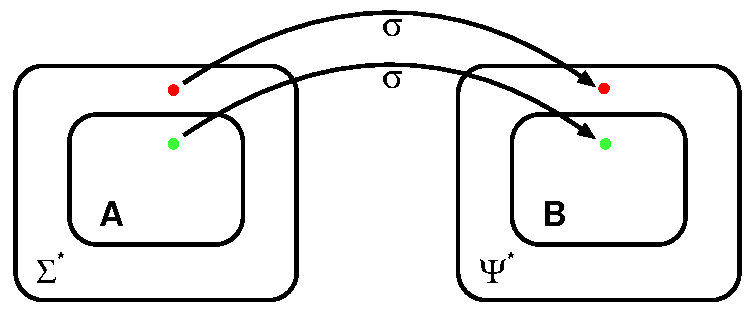
\includegraphics[width=0.75\linewidth]{redukce.pdf}
    \caption*{Redukce $\sigma : \Sigma^* \rightarrow \Psi^*$.}
\end{figure}

\paragraph*{Použití} \begin{compactitem}
    \item 1. směr: \begin{compactitem}
        \item Máme známý problém $P_1$, o kterém víme, že je (částečně) rozhodnutelný. To znamená, že existuje TS, který ho (částečně) rozhoduje.

        \item Máme nový problém $P_2$, o kterém chceme dokázat, že je (částečně) rozhodnutelný. Redukujeme $P_2$ na $P_1$.

        \item Cílem je najít takovou funkci $\sigma$ (překladač), která namapuje instance problému $P_2$ na instance problému $P_1$, takovým způsobem, že není porušena definice redukce.

        \item Z toho vyplývá, že je-li $P_1$ (částečně) rozhodnutelný, tak i $P_2$ je (částečně) rozhodnutelný.
    \end{compactitem}

    \begin{figure}[H]
        \centering
        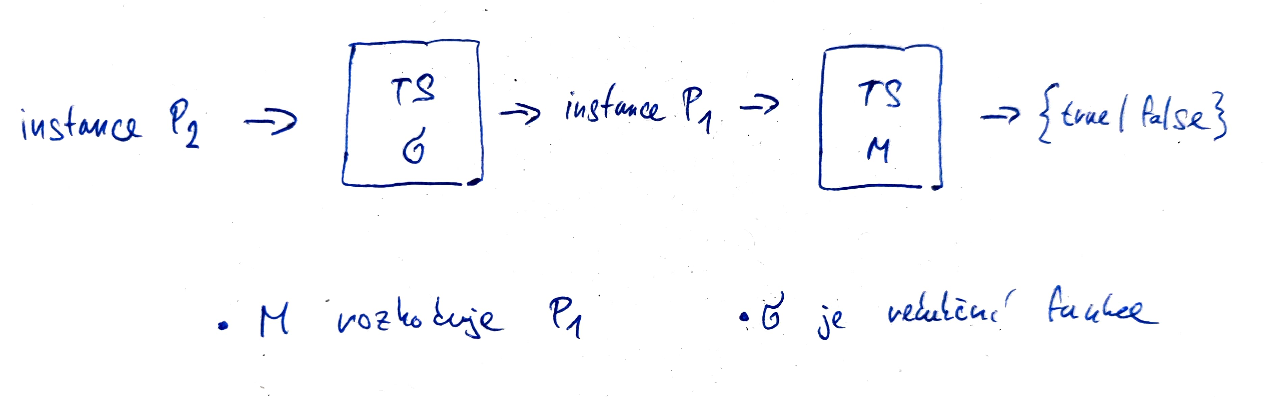
\includegraphics[width=1\linewidth]{redukce_1.pdf}
    \end{figure}

    \item 2. směr: \begin{compactitem}
        \item Máme známý problém $P_1$, o kterém víme, že je nerozhodnutelný (ani částečně).

        \item Máme nový problém $P_2$, o kterém chceme dokázat, že je nerozhodnutelný (ani částečně).

        \item Cílem je najít takovou funkci $\sigma$ (překladač), která namapuje instance problému $P_1$ na instance problému $P_2$, takovým způsobem, že není poručena definice redukce.

        \item Z toho vyplývá, že je-li $P_1$ nerozhodnutelný (ani částečně), tak i $P_2$ je nerozhodnutelný (ani částečně).
    \end{compactitem}

    \begin{figure}[H]
        \centering
        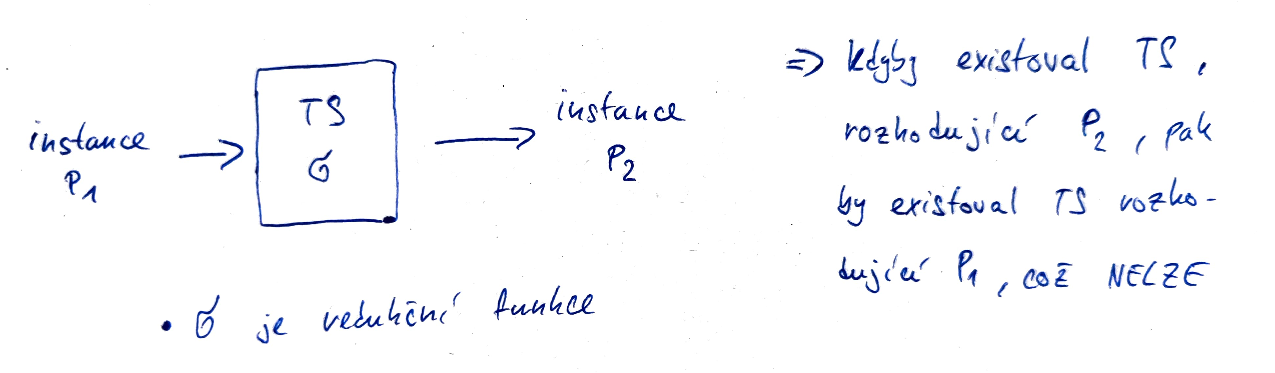
\includegraphics[width=1\linewidth]{redukce_2.pdf}
    \end{figure}
\end{compactitem}

\paragraph*{Obecný postup důkazu redukcí} \begin{compactenum}
    \item Navrhnout redukci.
    \item Ukázat, že redukce lze implementovat úplným TS.
    \item Ukázat, zachování členství v jazyce.
\end{compactenum}

\subsection*{Příklad 1: dokažte, že problém neprázdnosti jazyka TS je nerozhodnutelný}

\begin{compactitem}
    \item Dokážeme redukcí z problému zastavení TS (HP).

    \item Jazyk charakterizující problém zastavení (obsahuje takové instance, pro které TS $M$ na $w$ zastaví):
    $$ HP = \{ \langle M \rangle \# \langle w \rangle ~|~ \text{ TS } M \text{ na vstupu } w \text{ zastaví } \} $$

    \item Jazyk charakterizující problém neprázdnosti (obsahuje takové instance, pro které jazyk TS $M$ není prázdný):
    $$ NEMP = \{ \langle M \rangle ~|~ \text{M je TS takový, že } L(M) \not= \emptyset \} $$

    \item Navrhneme redukci (redukující HP na NEMP, viz směr 2, \uv{NEMP je aspoň tak těžký jako HP}):
    $$ HP \leq NEMP $$
    $$ \sigma : \{ 0, 1, \# \}^* \rightarrow \{ 0, 1 \}^* $$

    \item Funkce $\sigma$ přiřadí řetězci $x \in \{ 0, 1, \# \}^*$ řetězec $\langle M_{\sigma} \rangle$, kde $M_{\sigma}$ je TS implementující $\sigma$, pracující následovně: \begin{compactitem}
        \item $M_{\sigma}$ smaže svůj vstup (pozn. jazyk $L(M_{\sigma})$ tedy bude buď $\emptyset$ a nebo $\Sigma^*$).

        \item $M_{\sigma}$ zapíše na svůj vstup řetězez $x$.

        \item $M_{\sigma}$ ověří, zda $x = \{ \langle M \rangle \# \langle w \rangle \}$ má validní strukturu pro TS $M$ a jeho vstup $w$. Pokud nemá, tak odmítne.

        \item TS $M_{\sigma}$ odsimiluje běh TS $M$ na $w$. Pokud $M$ zastaví, tak přijme, jinak cyklí.
    \end{compactitem}

    \item Funkce $\sigma$ lze evidentně realizovat úplným TS $M_{\sigma}$. Skládá se, ze 4 komponent: \begin{compactenum}
        \item Smazání vstupu~--~konstantní operace, pro kterou $M_{\sigma}$ pouze vypíše daný kód.

        \item Zapsání $x$ na vstup~--~snadná operace, $M_{\sigma}$ vypíše kód, který provede přesun doprava a zápis $a_i$ pro $x = a_1 a_2 \dots a_n$ pro $i=1, 2, \dots, n$.

        \item Ověření správného strukturování vstupu~--~konstantní operace, pro kterou $M_{\sigma}$ pouze vypíše daný kód.

        \item Předání řízení univerzálnímu TS~--~konstantní operace, pro kterou $M_{\sigma}$ pouze vypíše daný kód.
    \end{compactenum}

    \item Ukázání zachování členství v jazyce. \begin{compactitem}
        \item Studujme jazyk $M_{\sigma}$: \begin{compactitem}
            \item $L(M_{\sigma}) = \emptyset \Leftrightarrow$ $x$ nemá validní strukturu $\langle M \rangle \# \langle w \rangle$ a nebo $M$ na $w$ nezastaví.

            \item $L(M_{\sigma}) = \Sigma^* \Leftrightarrow$ $x$ má validní strukturu $\langle M \rangle \# \langle w \rangle$ a $M$ na $w$ zastaví.
        \end{compactitem}
        \item Zachování členství:
        $$ \forall x \in \{ 0, 1, \# \}^* : \sigma(x) = \langle M_{\sigma} \rangle \in NEMP \Leftrightarrow $$
        $$ \Leftrightarrow L(M_{\sigma}) = \Sigma^* \Leftrightarrow $$
        $$ \Leftrightarrow x = \langle M \rangle \# \langle w \rangle \text{ a } M \text{ na } w \text{ zastaví } \Leftrightarrow $$
        $$ \Leftrightarrow x \in HP $$
    \end{compactitem}

\end{compactitem}

\subsection*{Příklad 2: dokažte, že problém prázdnosti jazyka TS není ani částečně rozhodnutelný}

\begin{compactitem}
    \item Dokážeme redukcí z problému nezastavení TS (coHP).

    \item Jazyk charakterizující problém nezastavení (obsahuje takové instance, pro které TS $M$ na $w$ nezastaví):
    $$ coHP = \{ \langle M \rangle \# \langle w \rangle ~|~ \text{ TS } M \text{ na vstupu } w \text{ nezastaví } \} $$

    \item Jazyk charakterizující problém prázdnosti (obsahuje takové instance, pro které jazyk TS $M$ je prázdný):
    $$ EMP = \{ \langle M \rangle ~|~ \text{M je TS takový, že } L(M) = \emptyset \} $$

    \item Navrhneme redukci (redukující coHP na EMP, viz směr 2, \uv{EMP je aspoň tak těžký jako coHP}):
    $$ coHP \leq EMP $$
    $$ \sigma : \{ 0, 1, \# \}^* \rightarrow \{ 0, 1 \}^* $$

    \item Funkce $\sigma$ přiřadí řetězci $x \in \{ 0, 1, \# \}^*$ řetězec $\langle M_{\sigma} \rangle$, kde $M_{\sigma}$ je TS implementující $\sigma$, pracující následovně: \begin{compactitem}
        \item $M_{\sigma}$ smaže svůj vstup (pozn. jazyk $L(M_{\sigma})$ tedy bude buď $\emptyset$ a nebo $\Sigma^*$).

        \item $M_{\sigma}$ zapíše na svůj vstup řetězez $x$.

        \item $M_{\sigma}$ ověří, zda $x = \{ \langle M \rangle \# \langle w \rangle \}$ má validní strukturu pro TS $M$ a jeho vstup $w$. Pokud nemá, tak přijme.

        \item TS $M_{\sigma}$ odsimiluje běh TS $M$ na $w$. Pokud $M$ zastaví, tak přijme, jinak cyklí.
    \end{compactitem}

    \item \textit{Zbytek na stejný princip jako v příkladu 1.}
\end{compactitem}

\subsection*{Příklad 3: dokažte, že problém náležitosti řetězce jazyku $L(M)$, kde M je TS, je nerozhodnutelný}

\begin{compactitem}
    \item Dokážeme redukcí z problému zastavení TS (HP).

    \item Jazyk charakterizující problém zastavení (obsahuje takové instance, pro které TS $M$ na $w$ zastaví):
    $$ HP = \{ \langle M \rangle \# \langle w \rangle ~|~ \text{ TS } M \text{ na vstupu } w \text{ zastaví } \} $$

    \item Jazyk charakterizující problém náležitosti řetězce jazyku $L(M)$, kde M je TS (obsahuje takové instance, pro které jazyk TS $M$ na $w$ zastaví a přijme):
    $$ MP = \{ \langle M \rangle \# \langle w \rangle ~|~ \text{M je TS takový, že } w \in L(M) \} $$

    \item Navrhneme redukci (redukující HP na MP, viz směr 2, \uv{MP je aspoň tak těžký jako HP}):
    $$ HP \leq MP $$
    $$ \sigma : \{ 0, 1, \# \}^* \rightarrow \{ 0, 1, \# \}^* $$
    $$ \sigma(\langle M \rangle \# \langle w \rangle) = \langle M' \rangle \# \langle w' \rangle $$

    \item Funkce $\sigma$ přiřadí řetězci $x \in \{ 0, 1, \# \}^*$ řetězec $\langle M \rangle \# \langle w \rangle$, kde $M_{\sigma}$ je TS implementující $\sigma$, pracující následovně: \begin{compactitem}

        \item $M_{\sigma}$ smaže svůj vstup (pozn. jazyk $L(M_{\sigma})$ tedy bude buď $\emptyset$ a nebo $\Sigma^*$).

        \item $M_{\sigma}$ zapíše na svůj vstup řetězez $x$.

        \item $M_{\sigma}$ ověří, zda $x = \{ \langle M \rangle \# \langle w \rangle \}$ má validní strukturu pro TS $M$ a jeho vstup $w$. Pokud nemá, tak \todo{todo: přijme?}.

        \item TS $M_{\sigma}$ odsimiluje běh TS $M$ na $w$. Pokud $M$ na $w$ zastaví přijme, tak $M_{\sigma}$ přijme. Jinak, $M_{\sigma}$ cyklí a nebo zamítá.
    \end{compactitem}

    \item \textit{Zbytek na stejný princip jako v příkladu 1.}
\end{compactitem}

\subsection*{Příklad 4: dokažte, že problém víceznačnosti bezkontextových gramatik, není ani částečně rozhodnutelný}

\todo{note: Příklad je na redukci z PCP, jedná se o těžší redukci, která se nebude zkoušet.}

%%%%%%%%%%%%%%%%%%%%%%%%%%%%%%%%%%%%%%%%%%%%%%%%%%%%%%%%%%%%%%%%%%%%%%%%%%%%%%%%
